%\documentstyle[amssymb,12pt,draft,epsf,palatino]{nature-pvd}
\documentclass{natureprintstyle}
\bibliographystyle{naturemag}

\usepackage{aas_macros}

\usepackage{epsfig,caption}
\usepackage{color}
\usepackage{bm}
\usepackage{graphicx}
\usepackage{longtable}
% \usepackage{amssymb}
\usepackage{rotating,xcolor}
\usepackage{hyperref}
% \usepackage{tgbonum}
\usepackage[symbol]{footmisc}
\usepackage{placeins}

\usepackage{amsmath}

\usepackage{fontspec}
\setmainfont{texgyrepagella}[
  Extension = .otf,
  UprightFont = *-regular,
  BoldFont = *-bold,
  ItalicFont = *-italic,
  BoldItalicFont = *-bolditalic,
]

\usepackage[misc]{ifsym}
\usepackage{xcolor}
\usepackage[labelfont=bf]{caption}
\DeclareCaptionLabelSeparator{lsep}{ | } 
\captionsetup{labelsep=lsep}


\newcommand{\RCR}{\ensuremath{R_{\textrm{CR}}}}
\newcommand{\Rot}{\ensuremath{\mathcal{R}}}

\newcommand{\Nbody}{$N$-body}
\newcommand{\Msun}{\ensuremath{M_{\odot}}}

\title{Stellar Bars in Isolated Gas-Rich Spiral Galaxies Do Not Slow Down}

\author{Angus~Beane$^{1*}$, Lars~Hernquist$^1$, Elena~D'Onghia$^{2,3}$,
Federico~Marinacci$^{4}$, Charlie~Conroy$^{1}$, Jia~Qi$^{5}$,
Laura~V.~Sales$^{6}$, Paul~Torrey$^{5}$ and Mark~Vogelsberger$^{7}$
}


\begin{document}

\maketitle

{\let\thefootnote\relax\footnote{

\begin{affiliations}
% 1
\item Center for Astrophysics $|$ Harvard \& Smithsonian,  Cambridge, MA, USA.

% 2
\item Department of Physics, University of Wisconsin-Madison, Madison, WI, USA.

% 3
\item Department of Astronomy, University of Wisconsin-Madison, Madison, WI, USA.

% 4
\item Department of Physics \& Astronomy `Augusto Righi', University of Bologna, Bologna, Italy.

% 5
\item Department of Astronomy, University of Florida, Gainesville, FL, USA.

% 6
\item Department of Physics \& Astronomy, University of California, Riverside, CA, USA.

% 7
\item Department of Physics, Massachusetts Institute of Technology, Cambridge, MA, USA.

$^{*}$ \texttt{\mbox{angus.beane@cfa.harvard.edu}}

\end{affiliations}
}}

% \renewcommand{\thefootnote}{\fnsymbol{footnote}}

\vspace{-3.5mm}
\begin{abstract}
  
  Elongated bar-like features are ubiquitous in galaxies, occurring at the
  centers of approximately two-thirds of spiral
  disks\cite{2000AJ....119..536E, 2007ApJ...657..790M}.  Due to gravitational
  interactions between the bar and the other components of galaxies, it is
  expected that angular momentum and matter will redistribute over long (Gyr)
  timescales in barred galaxies \cite{1972MNRAS.157....1L,
  1984MNRAS.209..729T, 1985MNRAS.213..451W}. Previous work ignoring the gas
  phase of galaxies has conclusively demonstrated that bars should slow their
  rotation over time due to their interaction with dark matter halos
  \cite{1992ApJ...400...80H, 2000ApJ...543..704D, 2002MNRAS.330...35A,
  2002ApJ...569L..83A, 2003MNRAS.341.1179A, 2003MNRAS.346..251O,
  2005MNRAS.363..991H, 2006ApJ...637..214M, 2007MNRAS.375..460W,
  2009ApJ...697..293D}. We have performed a simulation of a Milky Way-like
  galactic disk hosting a strong bar which includes a state-of-the-art model
  of the interstellar medium and a live dark matter halo. In this simulation
  the bar pattern does not slow down over time, and instead remains at a
  stable, constant rate of rotation. This behavior has been observed in
  previous simulations using more simplified models for the interstellar gas
  but its explanation has remained elusive\cite{1993AA...268...65F,
  2010ApJ...719.1470V}. We propose that the gas phase of the disk and the dark
  matter halo act in concert to stabilize the bar pattern speed and prevent a
  bar from slowing down or speeding up. We find that in a Milky Way-like disk,
  a gas fraction of only about \boldmath$5\%$ is necessary for this mechanism
  to operate. This result naturally explains why nearly all observed bars
  rotate rapidly\cite{2011MSAIS..18...23C, 2015AA...576A.102A,
  2019MNRAS.482.1733G} and is especially relevant for our understanding of how
  the Milky Way arrived at its present state.
  
\end{abstract}

\vspace{1cm}

%%%%%%%%%%%%%%%%%%%%%%%%%%%%%%%%%%%%%%%%%%%%%%%%%%%%%

\begin{figure*}[h!]%
\centering
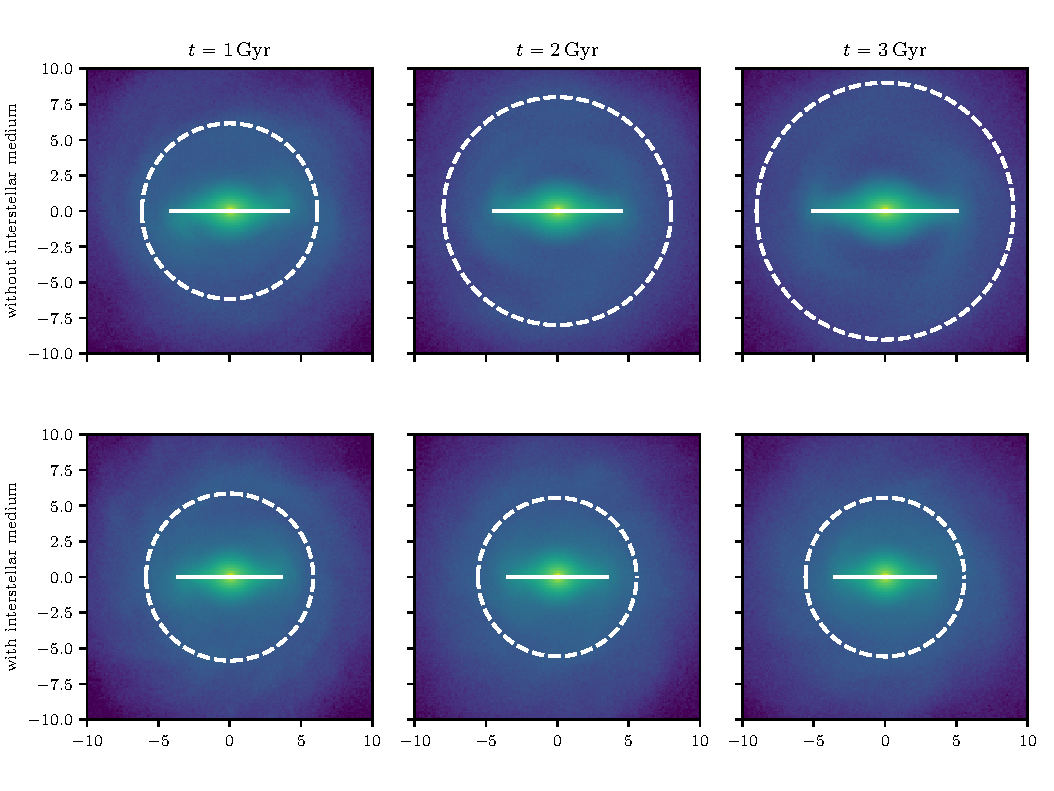
\includegraphics[width=18cm]{fig/fig1.pdf}
\caption{\textbf{Projected surface densities of simulated barred galaxies with
and without the interstellar medium.} The upper panels show an \Nbody{} only
simulation while the lower panels show a simulation which includes the SMUGGLE
model for the ISM. Columns show different points in time, separated by
$1\,\textrm{Gyr}$. We can see that in the \Nbody{} run, the bar grows in
length and strength. In the SMUGGLE run, the bar remains at approximately the
same length and strength over the course of the simulation. The \Nbody{} model
is identical to the GALAKOS model, discussed in the text.}\label{fig:overview}
\end{figure*}

\begin{figure}[h!]%
\centering
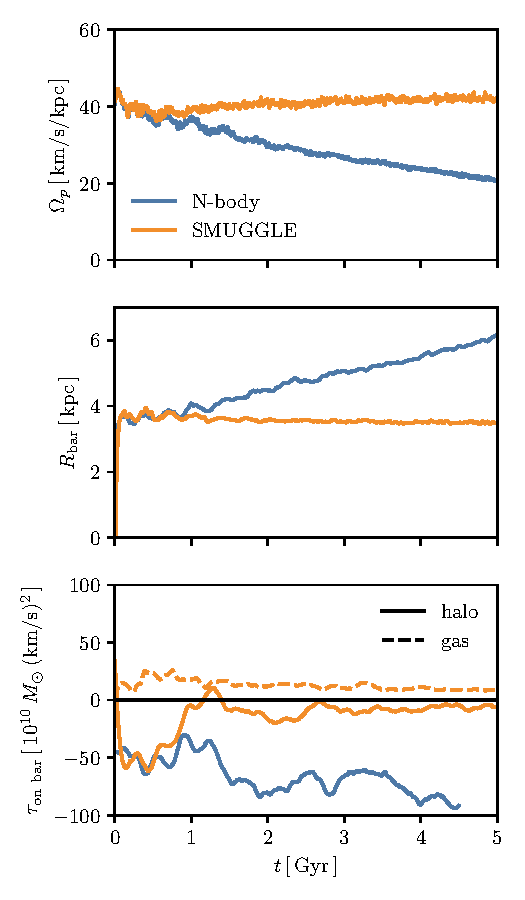
\includegraphics[width=9cm]{fig/fig2.pdf}
\caption{\textbf{Properties of the bar in our \boldmath$N$-body and SMUGGLE
simulations of a barred galaxy.} The \textit{upper panel} shows the evolution
of the pattern speed. As expected, the bar in the \Nbody{} run slows down due
to interactions between the bar and the dark matter halo. However, the bar in
the SMUGGLE run does not slow down and instead remains at a constant pattern
speed. The \textit{middle panel} shows the evolution of the bar length. In the
\Nbody{} case, the bar lengthens. This occurs because as the pattern speed
drops, bar-like orbits at larger radii are possible. Stars are captured on
these orbits, lengthening the bar. This process does not occur in the SMUGGLE
cases since the bar pattern speed is not decreasing, and therefore the bar
length remains constant. The \textit{lower panel} shows the torque on the bar
by different components. The solid lines show the torque exerted by the halo
in both the \Nbody{} and SMUGGLE cases. The dashed line shows the torque
exerted by the gas phase in the SMUGGLE run (there is no gas in the \Nbody{}
run). Details on how these properties are calculated is given in the Methods
section.}\label{fig:prop}
\end{figure}

\begin{figure*}[h!]%
\centering
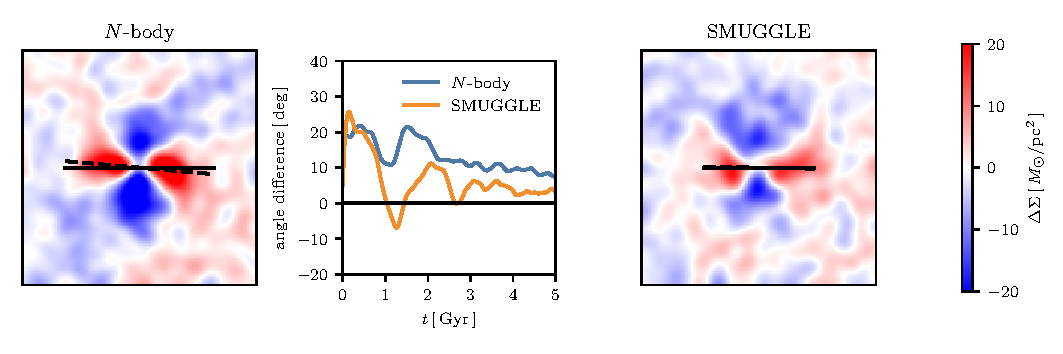
\includegraphics[width=18cm]{fig/fig3.pdf}
\caption{\textbf{The wake excited in the dark matter halo.} The dark matter
halo wake is shown in the \Nbody{} case (\textit{left panel}) and SMUGGLE case
(\textit{right panel}) after $2.6\,\textrm{Gyr}$ of evolution. The
\textit{left} and \textit{right panels} show a surface density projection in
the $x$-$y$ plane of the dark matter halo after an axisymmetric average has
been subracted. The solid line indicates the direction of the bar while the
dashed line indicates the direction of the halo wake (both measured by taking
the second Fourier component within a sphere of all material within a radius
of $4\,\textrm{kpc}$). The \textit{center panel} shows the time evolution of
the angle difference between the bar and the halo wake, as measured from the
second Fourier component. After the first Gyr, the angle difference in the
SMUGGLE case is smaller than in the \Nbody{} case by about a factor of two,
reflecting how the dark matter halo in the SMUGGLE case is unable to exert as
negative a torque on the bar as in the \Nbody{} case.}\label{fig:wake}
\end{figure*}

\begin{figure}[h!]
\centering
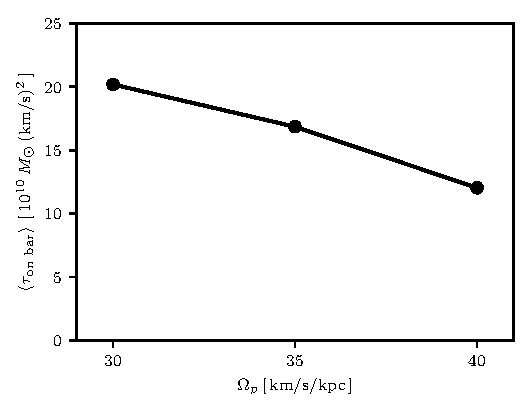
\includegraphics[width=9cm]{fig/fig4.pdf}
\caption{\textbf{Average torque exerted by gas on a bar which rotates at a
fixed pattern speed.} Since only gas within the corotation radius is able to
infall and slower bars have larger corotation radii, slower bars experience a
larger net torque than faster bars. The setup of the simulations used here is
identical to the SMUGGLE case discussed earlier and in the Methods section,
except the \Nbody{} disk is rotated as a solid body with a constant angular
velocity.}\label{fig:equil}
\end{figure}


It has long been known that non-axisymmetric features in a stellar disk act to
redistribute mass and angular momentum.\cite{1972MNRAS.157....1L} The
interaction between a bar and a spheroid (either a dark matter halo or stellar
bulge) has received considerable interest.\cite{1984MNRAS.209..729T,
1985MNRAS.213..451W} Stellar disks in isolation are prone to developing bars,
\cite{1971ApJ...168..343H} but the presence of a strong spherical potential
(e.g., from a stellar bulge or dark matter halo) acts to stabilize the disk
against bar formation.\cite{1973ApJ...186..467O, 1976AJ.....81...30H} Many
numerical simulations have confirmed that a live dark matter halo generically
exerts a negative torque on a bar, causing its pattern speed to decrease and
its length and strength to increase\cite{1992ApJ...400...80H,
2000ApJ...543..704D, 2002MNRAS.330...35A, 2002ApJ...569L..83A,
2003MNRAS.341.1179A, 2003MNRAS.346..251O, 2005MNRAS.363..991H,
2006ApJ...637..214M, 2007MNRAS.375..460W, 2009ApJ...697..293D}. Intuitively,
the bar excites a wake of resonant material in a dark matter halo in a manner
akin to dynamical friction. This wake lags a bar and thus exerts a negative
torque on it.

The expectation that a dark matter halo acts to slow down a bar is in
conflict with observational estimates of bar pattern speeds. Bar rotation
rates are typically classified by the dimensionless ratio
\begin{equation}
\Rot = \RCR/R_b\textrm{,}
\end{equation}
where \RCR{} is the radius of corotation and $R_b$ is the length of the
bar.\footnote{The radius of corotation \RCR{} is defined for circular orbits
as the radius at which the orbital frequency is equal to the pattern speed,
$\Omega_p$, of a given non-axisymmetric feature. In a galaxy with a constant
circular velocity $V_c$, it is given by $\RCR = V_c / \Omega_p$.} Galaxies
with $\Rot < 1.4$ are considered ``fast rotators'' while galaxies with $\Rot >
1.4$ are considered ``slow rotators.''\cite{2000ApJ...543..704D} Galaxies with
$\Rot < 1$ are not thought to be stable.\cite{1980AA....81..198C}
Observational estimates of the pattern speeds of bars indicate that nearly all
galaxies have $1 < \Rot < 1.4$.\cite{2011MSAIS..18...23C, 2015AA...576A.102A,
2019MNRAS.482.1733G}

The role of gas on the evolution of the bar is less well-understood. Since the
gas phase typically only contributes about $10-20\%$ of the mass of a galaxy
at the present day, one might naively expect it to have a subdominant effect
on the bar. However, because gas is collisional, it can participate in
non-resonant angular momentum exchange with the bar.\cite{2011MNRAS.415.1027H}
Thus, numerical work has shown that the gas phase can have a stronger
influence on a bar than its contribution to the mass of a galaxy would
suggest.\cite{2010ApJ...719.1470V, 2013MNRAS.429.1949A}

We have performed a simulation of a disk galaxy using the finite-volume
gravito-hydrodynamics code AREPO.\cite{2010MNRAS.401..791S} In AREPO, the
fluid is discretized as a moving Voronoi mesh. We use the additional physics
in the galaxy formation module Stars and MUltiphase Gas in GaLaxiEs (SMUGGLE)
\cite{2019MNRAS.489.4233M}. SMUGGLE is a comprehensive and self-consistent
galaxy formation model with a wide range of physical processes, including
radiative heating/cooling, star formation, and stellar feedback. More detailed
information on SMUGGLE is given in the Methods section. Our disk galaxy is a
modified version of the GALAKOS model\cite{2020ApJ...890..117D}, which
consists of a stellar disk, stellar bulge, and dark matter halo. After
$\sim2.5\,\textrm{Gyr}$ of evolution, the GALAKOS disk forms a bar consistent
with the Milky Way bar in terms of pattern speed and length
($\sim40\,\textrm{km}/\textrm{s}/\textrm{kpc}$ and $\sim4.5\,\textrm{kpc}$,
respectively). We modify this setup to include a gas phase, the details of
which are provided in the Methods section.

A surface density projection of our simulations is shown in
Fig.~\ref{fig:overview}. The upper three panels show the disk in the \Nbody{}
run while the lower three panels show the disk in the SMUGGLE run. Each column
shows the disk $\sim1\,\textrm{Gyr}$ apart in time. There is a large
qualitative difference in the evolution of the bar pattern between the two
runs. We see that in the \Nbody{} case, the bar lengthens in time and grows in
strength. In the SMUGGLE case, the bar retains a similar length and strength
between panels.

We show the time evolution of different bar properties in Fig.~\ref{fig:prop}.
In the upper panel, we show the pattern speed over time in the \Nbody{} (blue)
and SMUGGLE (orange) runs. The pattern speed in the \Nbody{} case slows down
while the pattern speed in the SMUGGLE case remains roughly constant. The
slowing down of the pattern speed in the \Nbody{} case is consistent with a long
line of numerical research on bars in \Nbody{}
simulations.\cite{1992ApJ...400...80H, 2000ApJ...543..704D,
2002MNRAS.330...35A, 2002ApJ...569L..83A, 2003MNRAS.341.1179A,
2003MNRAS.346..251O, 2005MNRAS.363..991H, 2006ApJ...637..214M,
2007MNRAS.375..460W, 2009ApJ...697..293D} However, in the SMUGGLE case the
pattern speed remains constant. After the first Gyr of evolution, we find that
the pattern speed increases by only $\sim10\%$ over the next
$4\,\textrm{Gyr}$, compared to a $\sim43\%$ decrease in the pattern speed for
the \Nbody{} run over the same interval. As we saw qualitatively in
Fig.~\ref{fig:overview}, the length of the bar in the \Nbody{} case grows over
time while it remains roughly constant in the SMUGGLE case. This is also
consistent with previous numerical work, which found that bars tend to grow as
they slow down and the radius of corotation
increases.\cite{2000ApJ...543..704D, 2003MNRAS.341.1179A}

The bottom panel of Fig.~\ref{fig:prop} shows the torque exerted on the bar by
different components. The solid lines indicate the torque on the bar by the
dark matter halo whereas the dashed line indicates the torque on the bar by
the gas phase. In the \Nbody{} case, the halo exerts a steady negative torque on
the bar, with an average torque from $1$ to $4\,\textrm{Gyr}$ of $-58.0$ in
units of $10^{10}M_{\odot}\,(\textrm{km}/\textrm{s})^2$. The halo in the
SMUGGLE case exerts a similar negative torque on the bar in the first Gyr of
evolution, but after that the halo exerts a much smaller torque on the bar,
averaging only $-7.8$ in the same units and over the same interval. The gas in
the SMUGGLE case exerts a steady positive torque averaging $11.7$ in the same
units and over the same interval.

The fact that the dark matter halo in the SMUGGLE case exerts a smaller
positive torque on the bar can be understood in terms of the halo wake
mechanism. In the \Nbody{} case, halo material which is resonant with the bar
will form a wake which lags behind and exerts a negative torque on the bar,
which slows it down.\cite{1984MNRAS.209..729T, 1985MNRAS.213..451W,
1992ApJ...400...80H}\footnote{Since the bar is not a solid body, it is not
guaranteed that a negative torque will slow it down - e.g. a negative torque
could shred the bar, reducing its moment of inertia without changing its
pattern speed. However, the bar seems to empirically respond to a negative
torque induced by a halo wake by slowing down.} As the bar slows down, the
location of the resonances in phase space changes, allowing halo material
newly resonant with the bar to participate in forming the wake. However, the
gas is a reliable source of positive torque on the bar, speeding the bar up.
This stops the resonance location from changing such that the halo cannot
reinforce a wake, arresting the process by which the halo can slow the bar
down.

We can test this interpretation by measuring the angle offset between the halo
wake and the bar. If the wake and the bar are aligned (i.e., there is no angle
offset), then the wake cannot exert a negative torque on the bar. This angle
is plotted in the middle panel of Fig.~\ref{fig:wake}, which shows that the
angle offset is larger in the \Nbody{} case than in the SMUGGLE case by about a
factor of two. The left and right panels of Fig.~\ref{fig:wake} show the halo
wake with respect to the location of the bar in the \Nbody{} (left) and SMUGGLE
(right) cases.

The presence of the gas can arrest the process by which additional material in
the dark matter halo can contribute to a wake. However, this does not explain
why the pattern speed in the SMUGGLE case is nearly constant over several Gyr.
Naively, it would be a coincidence that the bar pattern speed remains constant
in the SMUGGLE case, resulting from a chance cancellation of the halo and gas
torques. However, a constant pattern speed in the presence of gas has been
observed in a few simulations of barred galaxies with
gas.\cite{1993AA...268...65F, 2010ApJ...719.1470V} Previous work has argued
this is due to the bar torquing gas inwards, but no explanation has been given
for why it might remain constant.

We propose that an equilibrium mechanism is responsible for the pattern speed
remaining approximately constant. In this scenario, a torque must oppose
changes in the pattern speed so that when the bar speeds up, a negative torque
will slow it down and when the bar slows down, a positive torque will speed it
up. It is simple to explain the first of these - when the pattern speed
increases, the location of resonances will shift to regions of the dark matter
halo phase space where no wake has been excited yet (e.g., the corotation
radius will shrink).

When the bar slows down, we argue that this induces a larger positive torque
from the gas phase. Only gas within corotation will flow inwards, while gas
outside corotation will flow outwards.\cite{2011MNRAS.415.1027H} Since the
corotation radius is larger for more slowly rotating bars, it follows that
more slowly rotating bars should be more efficient at driving gas inflows and
thus experience a larger positive torque from the gas phase.

We performed an experiment to test this hypothesis by forcing the stellar disk
in the SMUGGLE run to rotate at a constant angular rate and measuring the
torque on the bar by the gas phase at different rotation rates. The result of
this experiment is shown in Fig.~\ref{fig:equil}, which shows that a more
slowly rotating bar experiences a larger positive torque from the gas. We have
therefore shown evidence for an equilibrium mechanism which keeps the pattern
speed of the bar constant, resulting from the complex interplay between the
dark matter halo and the gas phase.

We performed two additional tests to explore how our findings depend on the
assumed model of the interstellar medium and the amount of gas present in the
system. First, we performed a simulation of the same disk but with a simpler
model of the interstellar medium\cite{2003MNRAS.339..289S}, closer to standard
methods used in cosmological simulations of galaxy formation. We find that the
pattern speed evolution is nearly the same in this case, and so conclude that
our result is not sensitive to the details of the model for the interstellar
medium. The details of this experiment are given in the Methods section.

Second, we performed a set of simulations in which we decreased the initial
gas mass of the disk. We essentially find for our disk, our proposed mechanism
operates as long as the gas contributes about $5\%$ of the total mass of the
disk. If the gas available is below this threshold, then the pattern speed
will decrease in a similar fashion to standard \Nbody{} simulations.
Importantly, arbitrarily increasing the gas fraction does not cause the
pattern speed to continuously increase. This is consistent with our proposed
equilibrium mechanism and with previous studies of barred galaxies which
varied the gas fraction.\cite{2010ApJ...719.1470V} The exact critical gas
fraction above which our mechanism operates is likely dependent on the
properties of the bar, disk, and dark matter halo -- further work is needed to
characterize how this gas fraction varies with such properties. Details on
this test in which we varied the gas mass of the disk are given in the Methods
section.

The implications of our findings are numerous. First, we naturally explain why
nearly all observed galaxies are fast rotators without requiring the inner
regions of dark matter halos to be underdense\cite{1998ApJ...493L...5D,
2000ApJ...543..704D} or requiring new physics.\cite{2021MNRAS.503.2833R,
2021MNRAS.508..926R} Second, we show that the role of gas is of paramount
importance in studies which attempt to uncover the nature of dark matter from
its effect of slowing down the bar.\cite{2021MNRAS.500.4710C,
2021MNRAS.505.2412C} Third, we provide an explanation for how the Milky Way's
bar could be both long-lived and a fast rotator, of which there is some
observational evidence.\cite{2019MNRAS.490.4740B} And finally, we complicate
the picture of radial mixing expected to sculpt the Milky Way's disk
\cite{2012MNRAS.420..913B, 2015ApJ...808..132H}, a process which relies upon
the pattern speed of the bar to change with time (though our work does not
alter expectations for radial mixing induced by spiral
arms\cite{2002MNRAS.336..785S}).

Barred galaxies in cosmological simulations of galaxy formation continue to be
in conflict with observations by producing bars which rotate too
slowly.\cite{2017MNRAS.469.1054A, 2019MNRAS.483.2721P, 2021AA...650L..16F}
However, the pattern speeds of bars in both cosmological simulations and the
real universe can be affected by environmental processes not included in our
simulation -- e.g., satellite infall\cite{2011Natur.477..301P},
non-sphericity\cite{2013MNRAS.429.1949A} or rotation\cite{2013MNRAS.434.1287S,
2014ApJ...783L..18L, 2018MNRAS.476.1331C, 2019MNRAS.488.5788C} in the dark
matter halo, or perhaps even the gaseous circumgalactic medium. Naturally,
extending our present work to account for such effects is a crucial next step
in understanding the formation and evolution of galactic bars.

We found that below a certain gas fraction, bars should still be able to slow
down. Therefore, we expect barred spiral galaxies which are exceptionally
gas-poor to be rotating very slowly. We therefore predict that observations
which target such galaxies (e.g., lenticular barred
galaxies\cite{2009ARAA..47..159B}) would find slowly rotating bars. There does
exist one such example of a galaxy which is known to be a slow rotator -- the
low surface brightness galaxy UGC 628.\cite{2009AA...499L..25C} This galaxy
has been studied in detail by ref.\cite{2016MNRAS.463.1751C}, who note that it
indeed has a low gas fraction for galaxies of its type. In general, we predict
that bars in gas-rich spiral galaxies should rotate quickly while bars in
gas-poor spiral galaxies should rotate slowly.


%%%%%%%%%%%%%%%%%%%%%%%%%%%%%%%%%%%%%%%%%%%%%%%%%%%%

\bibliography{ref}

\begin{addendum}
  
\item [Acknowledgements] We would like to thank Greg~L. Bryan, Neal~J. Evans,
Drummond~B. Fielding, Keith Hawkins, Jason~A.~S. Hunt, Sarah~M.~R. Jeffreson,
Kathryn~V. Johnston, Peter~M.~W. Kalberla, Jürgen Kerp, Julio~F. Navarro,
Joshua~S. Speagle, David~N. Spergel, Martin~D. Weinberg, and Yanfei Zou for
helpful discussions. A.B. would like to thank Todd Phillips for helpful
discussions. Some computations in this paper were run on the FASRC Cannon
cluster supported by the FAS Division of Science Research Computing Group at
Harvard University. Resources supporting this work were also provided by the
NASA High-End Computing (HEC) Program through the NASA Advanced Supercomputing
(NAS) Division at Ames Research Center. A.B. was supported by the Future
Investigators in NASA Earth and Space Science and Technology (FINESST) award
number 80NSSC20K1536 during the completion of this work. L.H. funding. E.D.
funding. F.M. funding. C.C. funding. J.Q. funding. L.V.S. funding. P.T.
funding. M.V. funding.

\item[Author Contributions] Foo.

  \item[Data Availability] Foo.
    
  \item[Code Availability] A public version of the AREPO code is available at
  \url{https://arepo-code.org/}.
    
\end{addendum}


%%%%%%%%%%%%%%%%%%%%%%%%%%%%%%%%%%%%%%%%%%%%%%%%%%%%%%%%%%
%%%%%%%%%%%%%%%%%%%%%%%%%%%%%%%%%%%%%%%%%%%%%%%%%%%%%%%%%%

\FloatBarrier
\clearpage

\setcounter{page}{1}
\setcounter{figure}{0}
\setcounter{table}{0}
\renewcommand{\figurename}{Extended Data Figure}
\renewcommand{\thetable}{Extended Data \arabic{table}}

\noindent
{\bf \Large \uppercase{Methods} }

\bigskip

\noindent
{\bf Initial Setup}
\\
\noindent
The initial setup of the galactic disk used in this work follows closely the
GALAKOS model\cite{2020ApJ...890..117D}, which uses a modified version of
\texttt{MakeNewDisk}.\cite{2005MNRAS.361..776S} The GALAKOS model has three
components - a radially exponential and vertically isothermal stellar disk,
and a stellar bulge and dark matter halo following a Hernquist
profile.\cite{1990ApJ...356..359H} All \Nbody{} runs in this work used the same
setup parameters as the GALAKOS disk, more details of which can be found in
the original paper.

The addition of the gas phase was done as follows. The version of
\texttt{MakeNewDisk} used for the original GALAKOS model can generate a gas
disk which is radially exponential and in vertical gravito-hydrodynamic
balance. We modified the radial profile of this code in order to allow us to
generate a disk with a constant surface density within some cut-off radius,
and then exponentially declining beyond that radius with the scale-length of
the stellar disk. We used an initial surface density of
$20\,M_{\odot}/\textrm{pc}^2$ and a cut-off radius of $9.3\,\textrm{kpc}$.

After generating the gaseous disk in this way, we stitched the gas disk
together with the GALAKOS \Nbody{} disk (and bulge and dark matter halo) after
the GALAKOS disk has been allowed to evolve for $1.5\,\textrm{Gyr}$. The
purpose of allowing the GALAKOS disk to evolve first for a short period of
time is to allow for the bar to form unimpacted by the presence of the gas
(which would normally disrupt the formation of the bar). Throughout this work,
we consider $t=0$ for the \Nbody{} run to be the time at which we added the
gas phase for the SMUGGLE run (i.e. we ignore the first $1.5\,\textrm{Gyr}$ of
evolution of the \Nbody{} disk when the bar is forming). We made one
additional modification when stitching the gas disk together with the \Nbody{}
disk - we created a hole within the central $4\,\textrm{kpc}$. This hole
guards against an initial dramatic infall of gas within the bar region, which
we found to destroy the bar. Models of the Milky Way's gas surface density
profile indicate a reduction in gas in the bar region from $\sim1$ to
$\sim4\,\textrm{kpc}$,\cite{2022ApJ...929L..18E} and so our practice of
allowing the gas distribution to have a hole in the central region is
consistent with our choice to begin the simulations with a bar already formed.

\begin{figure}[t]%
\centering
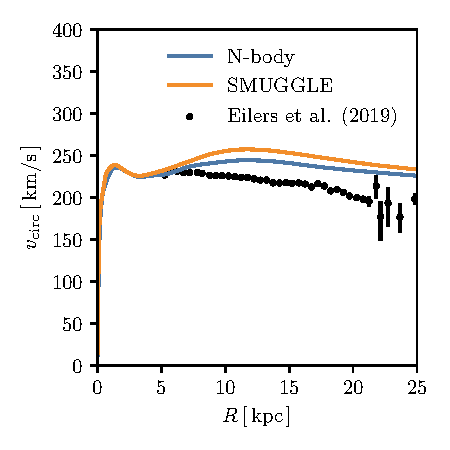
\includegraphics[width=9cm]{fig/fig-vcirc.pdf}
\caption{\textbf{The circular velocity curve of our initial setups.} This
curve is shown for the \Nbody{} run (blue) and the SMUGGLE run (orange)
compared to observational estimates for the Milky
Way.\cite{2019ApJ...871..120E} We see that the circular velocity curve for
both runs is marginally larger than the Milky Way's, but still comparable. The
SMUGGLE circular velocity curve is larger than the \Nbody{} curve due to the
additional mass in the gas phase.}
\label{fig:vcirc}
\end{figure}

\begin{figure}[h!]%
\centering
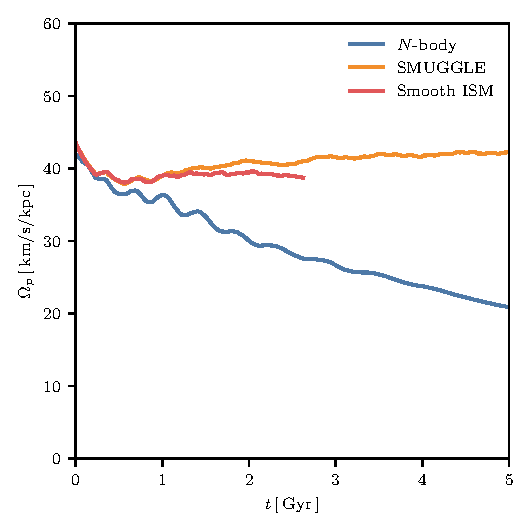
\includegraphics[width=9cm]{fig/fig-GFM.pdf}
\caption{\textbf{Pattern speed evolution of a smooth ISM model.} This
evolution is shown for the fiducial disk in the \Nbody{} (blue), SMUGGLE
(orange), and smooth ISM (red) cases. The smooth ISM model is an older model
for the ISM which treats its multiphase nature in a subgrid
fashion.\cite{2003MNRAS.339..289S} This fundamentally differs from the SMUGGLE
model, which explicitly resolve the hot and cold phases of the
ISM.\cite{2019MNRAS.489.4233M} The pattern speed in the smooth ISM case is
broadly similar to the evolution in the SMUGGLE case. This shows that the
stability of the pattern speed is not simply a result of our assumed model for
the ISM.}
\label{fig:GFM}
\end{figure}

Our setup is initially out of equilibrium, but we found that after
$\sim500\,\textrm{Myr}$, the entire system has settled into a steady-state
configuration and initial transients appear not to affect the results after
this point. The constant surface density of the initial gas disk is important
for ensuring the gas disk is dense enough in order for comparisons to real
galaxies to be appropriate.

We computed the circular velocity curve of our model using the \texttt{AGAMA}
package.\cite{2019MNRAS.482.1525V} We fit the baryonic component (stellar
disk, bulge, gas, and newly formed stars) with an axisymmetric cylindrical
spline with $20$ grid points in both the radial and vertical direction
spanning $0.2$ to $50\,\textrm{kpc}$ in the radial direction and from $0.02$
to $10\,\textrm{kpc}$ in the vertical direction. We fit the dark matter halo
using a spherically symmetric multipole fit with a maximum angular harmonic
coefficient of $l=2$. We plot the circular velocity curve in Extended Data
Fig.~\ref{fig:vcirc} compared to observational
estimates.\cite{2019ApJ...871..120E} Our disk is slightly more massive than
the Milky Way disk, and in the SMUGGLE run the addition of the gas phase
results in a slightly higher circular velocity. We also show the evolution of
the surface density profile in Extended Data Fig.~\ref{fig:surf} We find that
in our simulation the atomic and molecular gas surface density and the SFR
surface density is broadly consistent with the expected values for the Milky
Way.\cite{2008AA...487..951K,2022ApJ...929L..18E} The discrepancy between $1$
and $4\,\textrm{kpc}$ in the molecular and SFR surface density is likely due
to the fact that the distances to molecular clouds which underlines this work
used a simple kinematic distance based on an axisymmetric model of the Milky
Way,\cite{2017ApJ...834...57M} which is not accurate in the bar region
where gas has large non-circular velocities.

We used a mass resolution of $7.5\times10^3\,M_{\odot}$ for the baryonic
components (initial stellar disk, stellar bulge, and gas) and a mass
resolution of $3.75\times10^4\,M_{\odot}$ for the dark matter halo. This mass
resolution is closest to ``level 3'' in the AURIGA
simulations.\cite{2017MNRAS.467..179G} This corresponds to approximately
$6.4\times10^6$ particles in the stellar disk, $1.1\times10^6$ in the bulge,
$1.2\times10^6$ in the gas disk, and $25.3\times10^6$ in the dark matter halo.
We used a softening length of $0.02\,\textrm{kpc}$ for all components.
Snapshots were saved at equal intervals of $0.005$ in the time units of the
simulation ($\textrm{kpc}/(\textrm{km}/\textrm{s})\sim1\,\textrm{Gyr}$).

\begin{figure}[t!]%
\centering
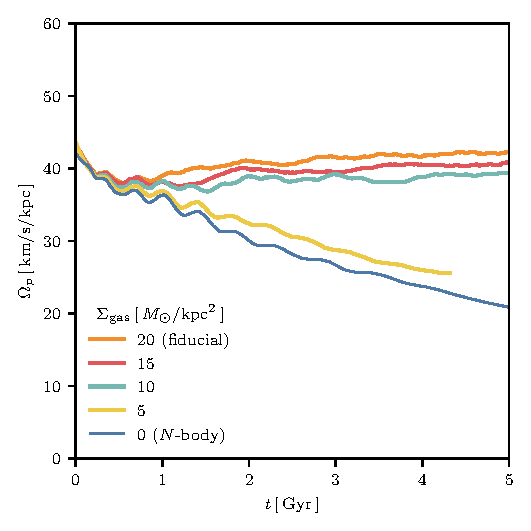
\includegraphics[width=9cm]{fig/fig-fgas.pdf}
\caption{\textbf{Pattern speed evolution with varying gas fractions.} We
explored the impact of lowering the initial gas surface density of our
fiducial disk on the evolution of the pattern speed. The surface densities we
tested of $20$, $15$, $10$, and $5\,\Msun/\textrm{kpc}^2$ correspond to
initial gas fractions of $16\%$, $10\%$, $7\%$, and $4\%$. We find that
initial surface densities $20$, $15$, and $10\,\Msun/\textrm{kpc}^2$ result in
bars which remain at a constant pattern speed, while an initial surface
density of $5\,\Msun/\textrm{kpc}^2$ results in a bar which slows down in
roughly the same manner as the \Nbody{} case. }
\label{fig:fgas}
\end{figure}

\begin{figure}[t!]%
\centering
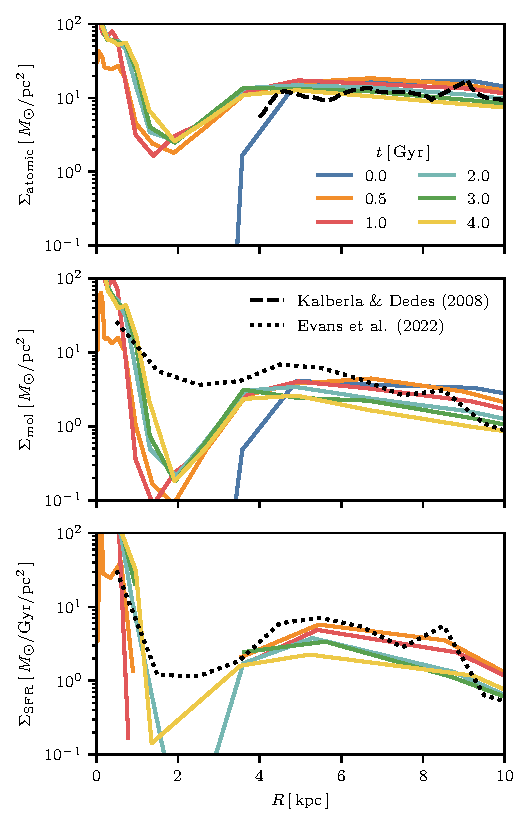
\includegraphics[width=9cm]{fig/fig-surf.pdf}
\caption{\textbf{Evolution of gas and SFR surface density profiles.} The time
evolution of the atomic gas surface density (\textit{upper}), molecular gas
surface density (\textit{middle}) and the star formation rate (SFR) surface
density (\textit{lower}) at various times during our fiducial simulation.
Colored lines indicate the profiles at selected times during the simulation
while the black dashed lines indicate observations for the atomic
gas\cite{2008AA...487..951K} and black dotted lines indicate a model which
allows the CO-to-H$_2$ conversion factor $X_{\textrm{CO}}$ to vary with
metallicity.\cite{2022ApJ...929L..18E} Molecular gas surface densities were
provided separately (N. Evans, private communication). We see that the
molecular gas and SFR surface densities are within an order of magnitude of
the Milky Way's typical values at all times.  We see a sharp decrease in the
gas and SFR surface densities along the extent of the bar from $\sim1$ to
$\sim4\,\textrm{kpc}$, related to the gas inflow in this region.}
\label{fig:surf}
\end{figure}

\vspace{12pt}

\noindent
{\bf SMUGGLE Model}
\\
\noindent
We use the Stars and MUltiphase Gas in GaLaxiEs (SMUGGLE) model
\cite{2019MNRAS.489.4233M} implemented within the moving-mesh, finite-volume
hydrodynamics code AREPO \cite{2010MNRAS.401..791S}. The SMUGGLE model
includes self-gravity, hydrodynamics, radiative heating and cooling, star
formation, and stellar feedback. Explicit gas cooling and heating of the
multi-phase interstellar medium is implemented, covering temperature ranges
between $10$ and $10^8\,\textrm{K}$.

Star formation occurs in cells above a density threshold
($n_{\textrm{th}}=100\,\textrm{cm}^{-3}$) according to
ref.\cite{2003MNRAS.339..289S} with a star-formation efficiency of $\epsilon =
0.01$. Star formation converts gas cells into star particles which represent
single stellar populations. For each star particle, the deposition of energy,
momentum, and mass from stellar winds and supernovae is modeled.
Photo-ionization and radiation pressure are modeled using an approximate
treatment. A more detailed description of this model can be found in the
flagship SMUGGLE paper.\cite{2019MNRAS.489.4233M}

We used the fiducial model parameters, except that we increased the number of
effective neighbors $N_{\textrm{ngb}}$ for the deposition of feedback from
$64$ to $512$. We found that a lower value of $N_{\textrm{ngb}}$ resulted in
inefficient photo-ionization feedback since the photo-ionizing budget had not
been exhausted after deposition into $64$ neighboring cells. We also used an
updated version of SMUGGLE using a new mechanical feedback routine similar to
the one described in ref.\cite{2018MNRAS.480..800H} This updated routine is a
tensor renormalization which ensures linear and angular momentum conservation
to machine precision.

\vspace{12pt}

\noindent
{\bf Smooth Interstellar Medium Model}
\\
\noindent
In addition to the SMUGGLE model, we considered a simpler model of the
interstellar medium based upon ref.\cite{2003MNRAS.339..289S} In this model,
the multiphase nature of the interstellar medium is modeled in a subgrid
manner by allowing each resolution element to have a ``cold'' and ``hot''
component, with the equation of state of the gas suitably modified. Gas is
allowed to interchange between the ``cold'' and ``hot'' components through
processes such as cooling and stellar feedback. Cold gas is allowed to undergo
star formation. The pattern speed evolution of this setup is given in Extended
Data Fig.~\ref{fig:GFM}, which shows that the pattern speed evolves in a
similar manner to the SMUGGLE case shown in Fig.~\ref{fig:prop}.

\vspace{12pt}

\noindent
{\bf Varying Gas Fraction}
\\
\noindent
We also performed a test in which we varied the initial gas fraction of the
disk. In our fiducial run, we set the surface density of the gas disk from
$4\,\textrm{kpc}$ to $\sim9.3\,\textrm{kpc}$ to be $20\,\Msun/\textrm{kpc}^2$.
We also ran with surface densities of $15$, $10$, and
$5\,\Msun/\textrm{kpc}^2$. These correspond to initial gas fractions of
approximately $16\%$, $10\%$, $7\%$, and $4\%$. The pattern speed evolution is
shown in Extended Data Fig.~\ref{fig:fgas} We find that the bar in disks with
initial surface densities of $20$, $15$, and $10\,\Msun/\textrm{kpc}$ evolve
with a constant pattern speed while the bar in a disk with initial surface
density of $5\,\Msun/\textrm{kpc}^2$ slows down at a similar rate to the \Nbody{} case.

As a result, we conclude that for the disk, bar, and halo properties
considered in this work, a gas fraction of only approximately $5\%$ is
necessary in order for the proposed stabilizing mechanism to operate. Furthermore, we co

\vspace{12pt}

\noindent
{\bf Bar analysis}
\\
\noindent
The analysis of various bar properties is performed as follows. First, the
pattern speed is measured from the angle of the second Fourier component. We
measured the second Fourier component by computing,
\begin{equation}
\begin{split}
A_2 &= \sum_i m_i e^{i 2 \phi_i} \\
A_0 &= \sum_i m_i \textrm{,}
\end{split}
\end{equation}
where $m_i$ and $\phi_i$ are the mass and azimuthal angle of each particle,
respectively. We computed $A_2$ and $A_0$ in cylindrical bins of width
$0.5\,\textrm{kpc}$ from radii of $0$ to $30\,\textrm{kpc}$. We defined the
angle of the bar $\phi_b$ to be twice the angle of the complex number $A_2$ as
measured in the bin extending from a radius of $2.5$ to $3\,\textrm{kpc}$.
After correcting for the periodicity of $\phi_b$, we measured the pattern
speed as the two-sided finite gradient of $\phi_b$ as a function of time.

\begin{figure}[t!]%
\centering
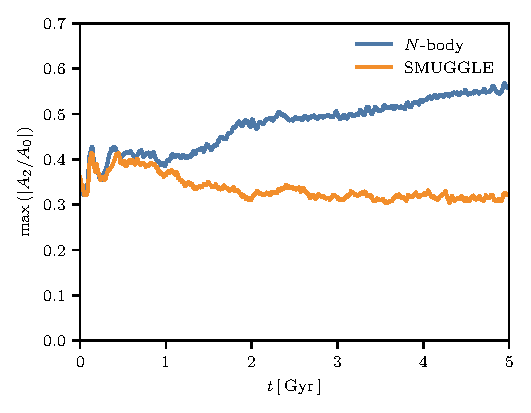
\includegraphics[width=9cm]{fig/fig-A2.pdf}
\caption{\textbf{Evolution of bar strength.} The bar strength is measured as
the maximum of the second Fourier component divided by the zeroth Fourier
component (a formula is given in the Methods section). We see that in the
\Nbody{} case (blue) the bar strength increases with time, consistent with
previous results showing that the bar strength increases as bars slow down. In
the SMUGGLE case (orange), we see that the bar strength remains roughly
constant, possibly slightly decreasing with time. This is also consistent with
the expected relation between pattern speed and strength since the bar in this
case is not slowing down.}
\label{fig:strength}
\end{figure}

\begin{figure*}[t!]%
\centering
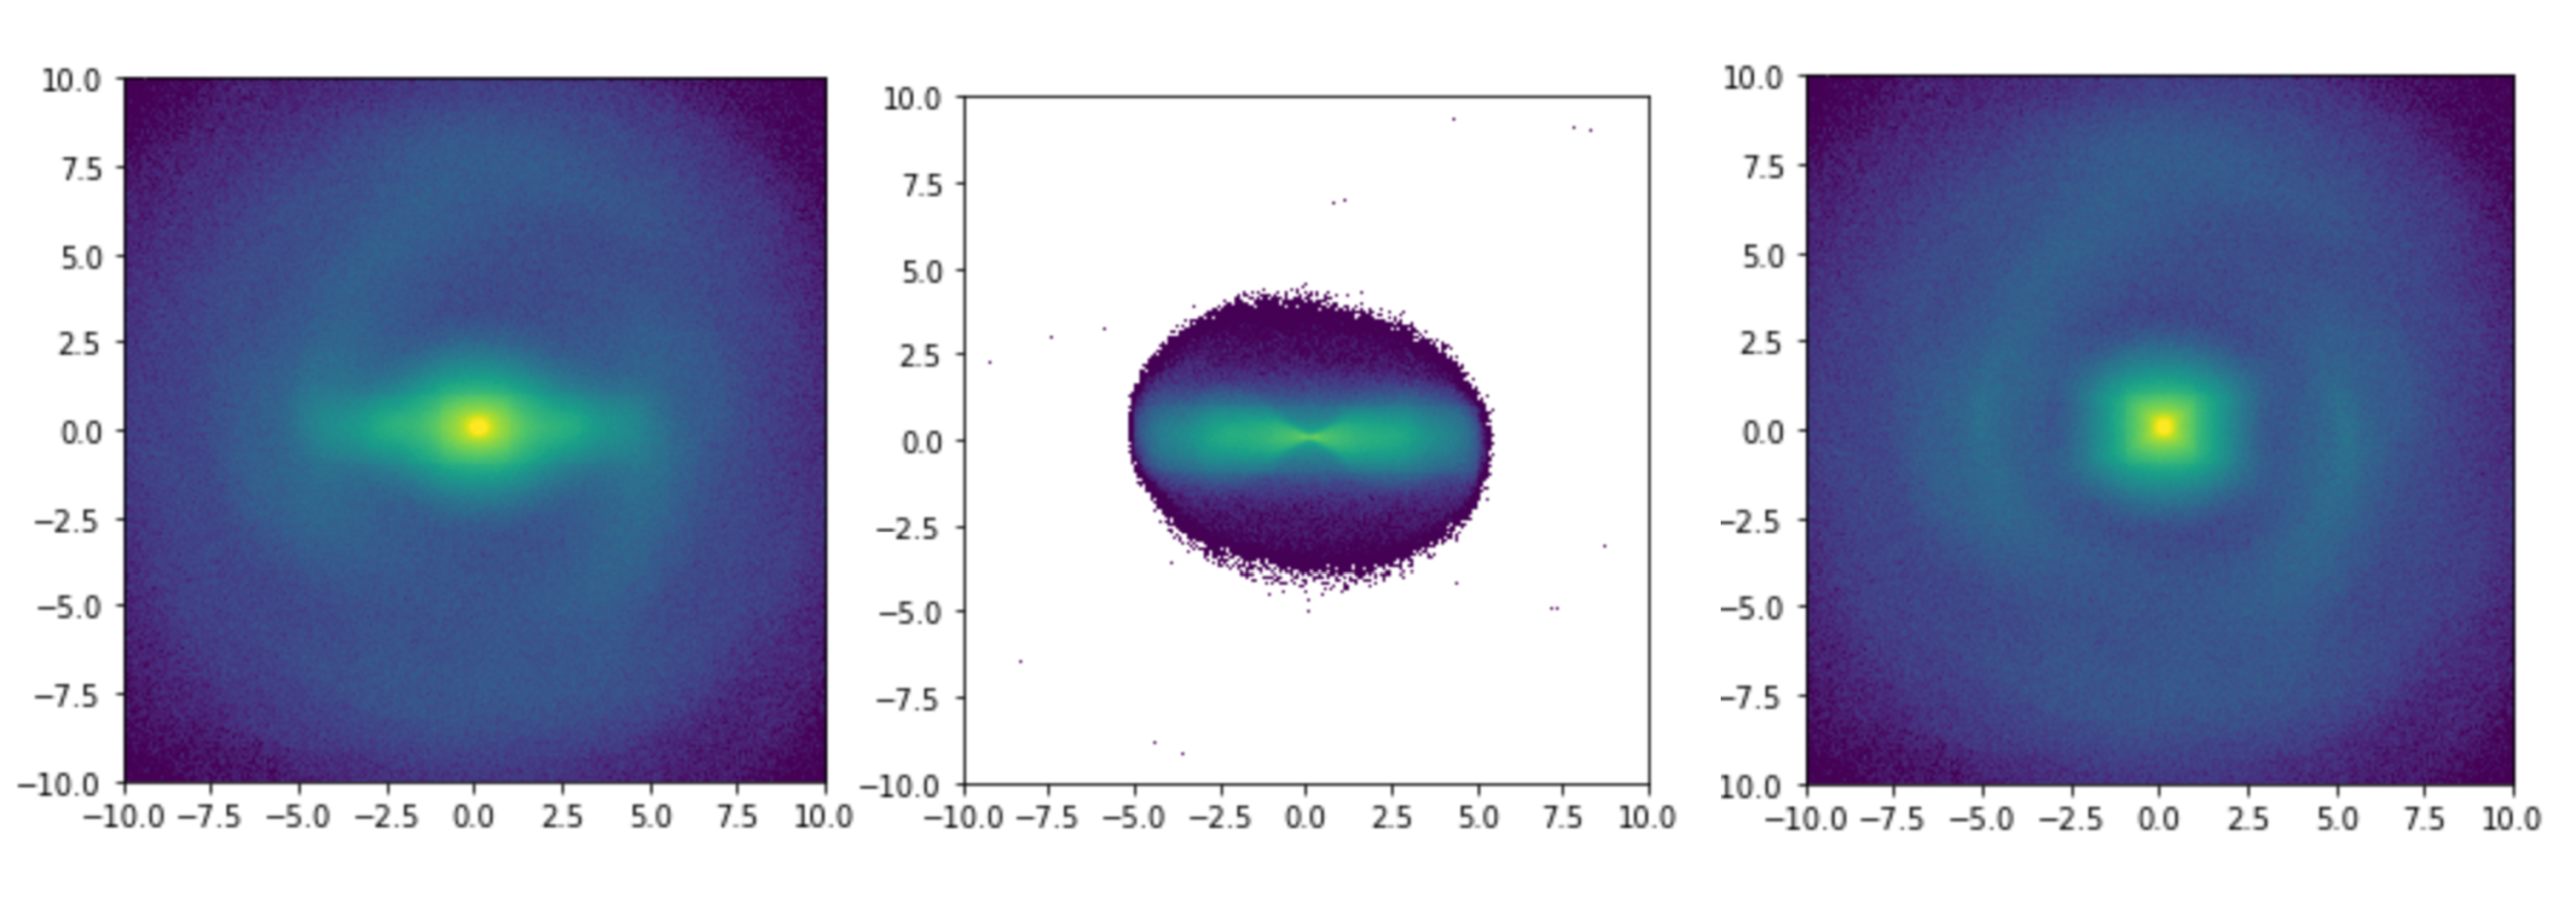
\includegraphics[width=18cm]{fig/fig-bar_decomp.pdf}
\caption{\textbf{Disk decomposition into the bar and unbarred disk.} This
procedure is based on ref.\cite{2016MNRAS.463.1952P} The \textit{left panel}
shows a surface density projection through the stellar component of the
\Nbody{} simulation (disk and bulge). The \textit{middle panel} shows the
component of the disk identified as being trapped in the bar while the
\textit{right panel} shows the component of the disk identified as not being
trapped in the bar. The fact that the untrapped stars form a roughly
axisymmetric structure indicates our bar decomposition is sufficiently
accurate. {\color{red} I will remake this figure
- I ended up losing the files which stored the bar membership, so I just
pulled these screenshots from an earlier presentation.}}
\label{fig:decomp}
\end{figure*}

The time evolution of the bar strength, defined as the maximum of
$\left|A_2/A_0\right|$ as a function of radius, is shown in Extended Data
Fig.~\ref{fig:strength}. The quantity $\left|A_2/A_0\right|$ varies from $0$
to $1$, with larger values indicating a stronger bar pattern. We see that in
the \Nbody{} case, $\left|A_2/A_0\right|$ increases over time as the bar pattern
slows. This is consistent with previous \Nbody{} simulations which showed a
clear correlation between the bar pattern speed and the bar
strength.\cite{2003MNRAS.341.1179A} In the SMUGGLE case, we see that the bar
strength has an initial drop but then remains at a roughly constant but
slightly decreasing strength. This is consistent with the pattern speed in the
SMUGGLE case being roughly constant or slightly increasing.

Computing the length of the bar and the torque on the bar by different
components requires us to decompose the disk into a component which is trapped
by the bar and a component which is untrapped. In order to do this, we follow
closely the technique developed in ref.\cite{2016MNRAS.463.1952P} We analyzed
the orbit of each star particle (meaning initial disk, bulge, and newly formed
stars) by extracting the $x$-$y$ positions of the apoapse of each in a frame
corotating with the bar (apoapses are defined as local maxima in $r$). For
each apoapse, we searched for the $19$ closest apoapses in time and applied a
$k$-means clustering algorithm on this set of $20$ points with $k=2$. We then
computed for each of the two clusters the average angle from the bar
$\left<\Delta \phi\right>_{0,1}$, the standard deviation in $R$ of the points
${\sigma_R}_{0,1}$, and the average radius of the cluster
$\left<R\right>_{0,1}$. At each apoapse, a particle was considered to be in
the bar if it met the following criteria:
\begin{equation}
\textrm{max}\left(\left<\Delta \phi\right>_{0,1}\right) < \pi / 8
\end{equation}
\begin{equation}
\frac{{\sigma_R}_0 + {\sigma_R}_1}{\left<R\right>_0 + \left<R\right>_1} < 0.22
\end{equation}
These criterion are slightly different and simplified from the ones used in
ref.\cite{2016MNRAS.463.1952P}, but we found to empirically work well at
decomposing the disk into a bar and disk component. In Extended Data
Fig.~\ref{fig:decomp}, we show an example of this decomposition. The
\textit{left} panel shows a surface density projection of the stellar disk and
bulge (including newly formed stars) from the SMUGGLE model after
$1\,\text{Gyr}$ of evolution in a frame such that the bar is aligned with the
$x$-axis. The \textit{middle} panel shows a projection of the subset of stars
that are identified as being trapped in the bar and the \textit{right} panel
shows a projection of the stars that are not identified as being trapped. The
fact that the \textit{right} panel is roughly axisymmetric indicates the bar
decomposition is performing adequately.

After the disk has been decomposed into a trapped and untrapped component, we
measured the bar length as being the radius $R_b$ which encapsulates $99\%$ of
the stars identified as being trapped in the bar, allowing for some outliers.
For the computation of the torque, we used the tree algorithm in
\texttt{MakeNewDisk}\cite{2005MNRAS.361..776S} customized to be accessible
from \texttt{Python} using \texttt{Cython}. This algorithm is based on the
\texttt{TREESPH} code.\cite{1989ApJS...70..419H} We constructed a tree using
only the star particles identified as being trapped in the bar using an
opening angle of $0.35$. We then queried the tree at the locations of all
resolution elements in the other components and computed the torque of the bar
on such components. The torque on the bar by the other components is simply
the negative of the torque on the other components by the bar. A similar
method was applied in measuring the torque for the disk when the pattern speed
is kept constant, as is done in Fig.~\ref{fig:equil}.

\vspace{12pt}

\noindent
{\bf Plotting Details}
\\
\noindent
We saved snapshots in intervals of $0.005$ in the time units of the
simulation, $\textrm{kpc}/(\textrm{km}/\textrm{s})$, which is very nearly
equal to $1\,\textrm{Gyr}$ (it is $\sim0.977\,\textrm{Gyr}$). Therefore,
throughout this work we referred to the native code time unit as
$\textrm{Gyr}$. None of our results are sensitive to this choice.

In order to remove numerical noise in several quantities we computed, we
applied a Savitzky-Golay filter\cite{1964AnaCh..36.1627S} as implemented in
\texttt{scipy} using a window length of $81$ and polynomial order of $3$. This
filter was applied to plots of pattern speeds, bar lengths and strengths,
torques, and angle differences.

% \bibliography{ref2}



\end{document}



% 